\begin{center}
\chapter{Chapter 04}
\end{center}
\vspace{11mm}
\section{Implementation and Testing}
\subection{Introduction}
The Blood Bank Android programmer Project Report's Implementation and Testing section concentrates on the actual creation of the programmer and the extensive testing carried out to guarantee its dependability. Coding, feature integration, and user interface design are all part of this phase and are done in accordance with the identified criteria. The section introduces the development methodology used, such as Waterfall or Agile, and places emphasis on the value of testing in identifying and fixing flaws. To verify that the programmer complies with requirements, several testing approaches are used, such as unit testing and user acceptability testing. A stable and user-friendly Blood Bank Android Application that is prepared to successfully meet the issues in the blood donation procedure is the result of successful implementation and extensive testing.
\subsection{System Setup}
Android Studio, Java, and Firebase as the bacERkend database were used to successfully construct the Android-based Blood Bank Project with OTP sign-in option. In order to enable smooth user authentication using phone number sign-in with OTP, Firebase Authentication and Realtime Database had to be integrated into the system's setup. The project offers a user-friendly interface with well-designed XML layouts for tasks like sign-in, sign-up, dashboard, and blood donation form. Users may register, sign in using an OTP, and donate blood by providing their donation information to the Firebase Realtime Database thanks to the Java code's efficient handling of user authentication and database operations. The application has undergone extensive testing and debugging to guarantee its dependability, compatibility, and responsiveness on different Android devices. The application is prepared for distribution on the Google Play Store or for testing, with a focus on data security and error management. In addition to streamlining the blood donation procedure, this Android-based Blood Bank Project with OTP sign-in support and Java and Firebase Database promises to favourably impact the healthcare industry by enticing more people to donate blood and save lives.
\newpage
\subsection{Data Flow Diagram}
The Blood Bank Android Application Project Report includes a Data Flow Diagram (DFD) that graphically illustrates data flow and user interactions. Data sources, processes, and data repositories make up its three key parts. Data sources include user input like registration information and information about blood donations. User registration is required for validation, and donor-recipient matching is required for effective blood donation. User data and records of blood donations are kept in data stores. The arrows show how data flows smoothly across components, showing how user input gets to the appropriate procedures and data repositories. Understanding the data flow of the application and simplifying decision-making during development are both made easier with the help of the DFD.

\begin{figure}[h]
    \centering
    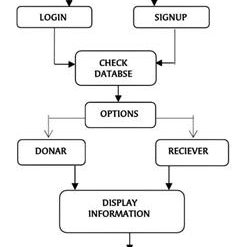
\includegraphics[height=12cm]{img/dfd.jpg}
    \caption{Data Flow Diagram}
    \label{fig:enter-label}
\end{figure}

\subsection{Result and Discussion}
The Blood Bank Android Application Project Report's Result and Discussion part provides a thorough overview of the project's results and conclusions. Beginning with the successful implementation of important application functions, such as user registration, donor-recipient matching, real-time notifications, and blood donation tracking, the section goes on to discuss these aspects in more detail. It validates the simple OTP sign-in process for user authentication, guaranteeing registered users secure access. It is also described how well the Firebase Realtime Database works to store and retrieve information about users, donors, and blood donations. The impact of the application on blood donation procedures is also covered in the conversation. It assesses how the application has increased blood accessibility by enabling prompt and effective matching of donors and recipients. The segment also looks at how the programmer might speed up crucial medical procedures and emergency response times, making healthcare services more effective.
The project's difficulties and constraints are openly discussed, along with suggested solutions or areas for improvement. To make sure the application conforms with industry standards and user expectations, data privacy and security measures are inspected.The part investigates the application's scalability and potential future improvements. Based on user feedback and identified areas for improvement, it takes feature extension options into consideration. The Conclusion highlights the Blood Bank Android Application project's overall accomplishments and highlights the good effects it has had on blood donation procedures and healthcare services.
 
\begin{figure}[h]
    \centering
    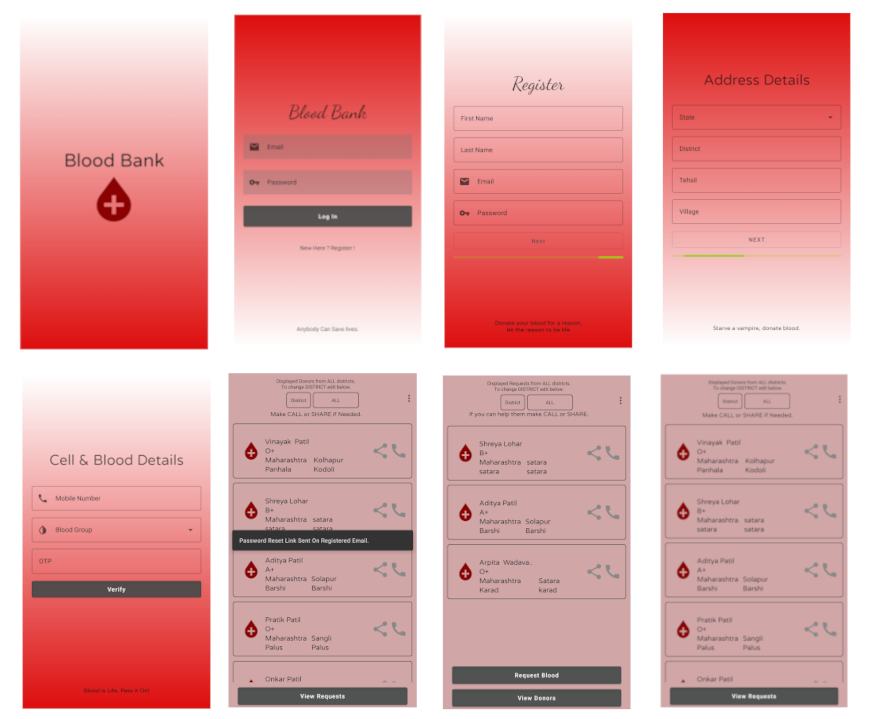
\includegraphics[ width=6cm]{img/bloodBankProject.png}
    \caption{Blood Bank Apps UI}
    \label{fig:enter-label}
\end{figure}

\subsection{Summary}
The Blood Bank Android Application Project Report's Implementation and Testing Summary shows the efficient creation and integration of crucial features including user registration, donor-recipient matching, and real-time notifications utilising Firebase. The application's functionality and user-friendliness were ensured through the testing procedure, which also included unit testing and user acceptance testing. Bugs and problems were fixed, which improved the stability and functionality of the application. The Blood Bank Android Application is now ready for deployment and acceptance and has the potential to enhance blood donation procedures and healthcare services, according to user input.
